\documentclass[conference]{IEEEtran}
\IEEEoverridecommandlockouts

\usepackage{cite}
\usepackage{amsmath,amssymb,amsfonts}
\usepackage{graphicx}
\graphicspath{{figuras/}}
\usepackage{textcomp}
\usepackage{xcolor}
\usepackage{booktabs}
\usepackage{multirow}
\usepackage{array}
\usepackage[output-decimal-marker={,}]{siunitx}
\usepackage[hidelinks]{hyperref}
\usepackage{float}
\usepackage{caption}
\usepackage{placeins}
\usepackage{tikz}
\usetikzlibrary{positioning,arrows.meta,calc}

\renewcommand{\tablename}{TABLA}
\renewcommand{\figurename}{Fig.}
\renewcommand{\abstractname}{Resumen}
\renewcommand{\refname}{Referencias}
\renewcommand{\IEEEkeywordsname}{Palabras clave}

\begin{document}

\title{Diseño de una Fuente de Alimentación Lineal Regulada de $\pm$16~V / 1,5~A y +5~V con Protección Foldback para los Controladores PID Analógicos de un Levitador Magnético}

\author{
\IEEEauthorblockN{Brahiam Alberto Campiño Romero}
\IEEEauthorblockA{\textit{Programa de Ingeniería Electrónica} \\
\textit{Universidad de Ibagué}\\
Ibagué-Tolima, Colombia \\
brahiam.campino@estudiantesunibague.edu.co}
}

\maketitle

\begin{abstract}
Se diseña, simula y lleva a placa una fuente lineal que entrega $+16$~V y $-16$~V, cada una capaz de 1,5~A, y $+5$~V, para alimentar los cuatro controladores PID analógicos de un levitador magnético y para demostrar la corriente de especificación sobre una carga de prueba removible. El método es el del tema 3 de la monografía \emph{Electrónica Tomo II}~\cite{monografia}: transformador, rectificador, filtro y regulador, con regulación de línea, regulación de carga, factor de rizado y protecciones. Como los reguladores LM317 y LM337 no podían cambiarse, su capacidad se amplía con un transistor de potencia (Fig.~3-21 de la monografía), de modo que el integrado conduzca solo una cuarta parte de la corriente. Antes de cada regulador hay un limitador de corriente con transistor Darlington y protección \emph{foldback} (Figs.~3-26 y 3-27): limita a unos 2,4~A en sobrecarga y reduce la corriente de cortocircuito a 0,8--1,2~A, y está ajustado para que la carga de prueba no lo deje trabado al arrancar. Un transformador de 18-0-18~V / 3~A con puente rectificador alimenta los dos rieles, y se reutilizan capacitores de $\SI{15000}{\micro F}$ y $2\times\SI{6800}{\micro F}$. La simulación en ngspice muestra salidas de $\pm15{,}98$~V con 1,6~A, regulación de carga del 0,09~\%, rizado de salida de 0,1~mV$_{pp}$, regulación aun con la red al $-10$~\%, y recuperación automática tras cortocircuitos sostenidos. Se entregan los esquemáticos, los archivos EAGLE/Fusion de una placa de una cara de $190\times140$~mm, la lista de materiales y el plan de pruebas.
\end{abstract}

\begin{IEEEkeywords}
fuente lineal, LM317, LM337, ampliación de corriente, foldback, limitador de corriente, puente rectificador, regulación de carga, levitación magnética
\end{IEEEkeywords}

% =========================================================
\section{Introducción}
% =========================================================
El levitador magnético del proyecto usa cuatro controladores PID analógicos idénticos, uno por bobina. Cada uno tiene dos TL074CN, un sensor Hall SS495A y un divisor que genera la referencia $V_{ref}=2$~V a partir de $+5$~V~\cite{informepid}. Los amplificadores se alimentan con $\pm16$~V, el divisor y los sensores con $+5$~V, y las bobinas con una fuente aparte, cuyo negativo (PGND) se une a la tierra de señal en un solo punto.

La primera versión de esta fuente se dimensionó solo para los operacionales: 0,27~A por riel con el transformador M509 disponible. Después se agregó una especificación: la fuente debe entregar \textbf{1,5~A en los rieles de $\pm16$~V} sobre una carga de prueba que pueda conectarse y desconectarse, para medir con y sin carga. Además, debía \textbf{conservar las protecciones} y usar los mismos reguladores LM317 y LM337, porque no había tiempo para conseguir otros. Este informe documenta el diseño definitivo (versión 2) y explica qué cambió y por qué.

El método es el del tema 3 de la monografía~\cite{monografia}. La fuente se divide en los bloques de su Fig.~3-1: transformador, rectificador, filtro y regulador. Los parámetros se definen como allí: voltaje y corriente de salida, regulación de línea ante $\pm10$~\%, regulación de carga, factor de rizado y coeficiente de temperatura. Las topologías y los criterios de diseño también son los de la monografía.

% =========================================================
\section{Objetivos}
% =========================================================
\subsection{Objetivo general}
Diseñar una fuente lineal regulada de $\pm16$~V / 1,5~A y $+5$~V, con protección contra cortocircuito, que alimente los cuatro controladores PID del levitador y permita demostrar la corriente de especificación sobre una carga removible, siguiendo el método de la monografía \emph{Electrónica Tomo II}.

\subsection{Objetivos específicos}
\begin{itemize}
\item Dimensionar el transformador, el rectificador y el filtro para 1,5~A, reutilizando los capacitores disponibles.
\item Ampliar la corriente de los reguladores LM317/LM337 sin reemplazarlos.
\item Diseñar una protección contra cortocircuito que soporte un corto sostenido y que no se trabe al arrancar con la carga de prueba.
\item Dimensionar disipadores y fusibles.
\item Comprobar el diseño por simulación: régimen, línea, carga, cortocircuito, arranque y curva V--I.
\item Entregar la placa, la lista de materiales y el plan de pruebas.
\end{itemize}

% =========================================================
\section{Especificaciones}
% =========================================================
\subsection{Corrientes}
Los cuatro PID consumen hasta 200~mA en cada riel de $\pm16$~V (50~mA por PID, con margen~\cite{tl074}). La rama de $+5$~V consume 57~mA: cuatro sensores de 10~mA~\cite{ss495a}, los divisores, la red de ajuste de su regulador y un LED. La especificación de 1,5~A se comprueba con una resistencia externa $R_L=\SI{10}{\ohm}$ en la bornera J4 ($+16$~V) o J5 ($-16$~V), que da $16/10=1{,}6$~A. A esa corriente se suma el consumo interno de cada riel (red de ajuste, LED y, en $+16$~V, la rama de $+5$~V):
\begin{align}
I_{L(+16)}&=1{,}6+0{,}017+0{,}057=\SI{1,674}{A},\\
I_{L(-16)}&=1{,}6+0{,}017=\SI{1,617}{A}.
\end{align}
La carga de 1,5~A se prueba \textbf{en un riel a la vez}, y con eso se dimensiona el transformador.

\begin{table}[htbp]
\caption{Especificaciones de la fuente (versión 2)}
\label{tab:espec}
\centering
\footnotesize
\begin{tabular}{@{}lccc@{}}
\toprule
Parámetro & +16~V & $-16$~V & +5~V \\
\midrule
Ajuste de salida & \multicolumn{2}{c}{$\pm$15 a $\pm$17~V} & 4,7 a 5,2~V \\
Corriente nominal & 1,5~A ($R_L$) & 1,5~A ($R_L$) & 57~mA \\
Límite en sobrecarga & \multicolumn{2}{c}{$\approx$2,4~A} & $\approx$90~mA \\
Corriente de corto & \multicolumn{2}{c}{$\leq$1,2~A (foldback)} & 0,145~A \\
Regulación de carga & \multicolumn{3}{c}{$\leq$0,5~\%} \\
Regulación de línea ($\pm10$~\%) & \multicolumn{3}{c}{$\leq$0,2~\% de $V_{out}$} \\
Rizado de salida & \multicolumn{3}{c}{$<$1~mV$_{pp}$} \\
Entrada & \multicolumn{3}{c}{115~V$_{rms}$ $\pm$10~\%, 60~Hz} \\
\bottomrule
\end{tabular}
\end{table}

% =========================================================
\section{Marco teórico}
% =========================================================
\subsection{Parámetros de la fuente}
La fuente regulada (Fig.~3-1 de~\cite{monografia}) está formada por transformador, rectificador, filtro y regulador. La monografía la caracteriza con cuatro parámetros: voltaje y corriente de salida, regulación (de línea, ante $\pm10$~\% de $V_{in}$, y de carga), factor de rizado $F_r=V_{r(rms)}/V_{DC}$ y coeficiente de temperatura. La regulación de carga se define como
\begin{equation}
\%\,\text{Regulación}=\frac{|V_{ro}|-|V_r|}{|V_r|}\times100\,\%,
\label{eq:reg}
\end{equation}
con $V_{ro}$ la salida en vacío y $V_r$ a plena carga.

\subsection{Regulador ajustable}
El LM317 mantiene $V_A=1{,}25$~V entre OUT y ADJ, y por ADJ sale una corriente $I_Q\approx\SI{50}{\micro A}$~\cite{lm317}. Con $R_1$ entre OUT y ADJ y $R_2$ de ADJ a tierra (ec.~(3.19) de~\cite{monografia}):
\begin{equation}
V_{out}=V_A\left(1+\frac{R_2}{R_1}\right)+I_Q R_2 .
\label{eq:vout}
\end{equation}
El LM337 es su complemento negativo~\cite{lm337}.

\subsection{Ampliación de corriente}
La monografía amplía la corriente de un regulador integrado con un transistor de paso PNP (Fig.~3-21). La corriente de entrada del regulador, $I_U$, pasa por una resistencia $R$ conectada entre la base y el emisor del transistor. Cuando $I_U R$ llega a $V_{BE}$, el transistor conduce y aporta la corriente que falta:
\begin{equation}
I_L=I_{C1}+I_U,\qquad R=\frac{V_{BE}}{I_U-I_B}.
\label{eq:booster}
\end{equation}
El regulador sigue fijando la tensión de salida, y la monografía recomienda que $I_U$ sea menor que el 50~\% de la corriente máxima del regulador.

\subsection{Limitación de corriente y foldback}
En el limitador con transistor (Figs.~3-24b y 3-26), la corriente pasa por $R_{SC}$, conectada entre la base y el emisor de un transistor sensor. Cuando $I R_{SC}\geq V_{BE}$, el sensor le quita la corriente de base al transistor de paso:
\begin{equation}
R_{SC}=\frac{V_{BE}}{I_{L(max)}} .
\label{eq:rsc}
\end{equation}
En un corto sostenido, el transistor de paso disipa $V_{in}I_{L(max)}$. El limitador \emph{foldback} (Fig.~3-27) suma al sensor una fracción $k$ de una tensión que cae cuando la salida colapsa. Así la corriente de corto $I_{SC}$ queda por debajo de la corriente máxima $I_{FB}$ (ecs.~(3.33)--(3.35)):
\begin{equation}
I_{SC}=\frac{V_{BE}}{kR_{SC}},\qquad I_{FB}=I_{SC}+\frac{(1-k)V_{out}}{kR_{SC}} .
\label{eq:fb}
\end{equation}

% =========================================================
\section{Diseño paso a paso}
% =========================================================
\subsection{Historial de versiones}
\label{sec:hist}
La Tabla~\ref{tab:versiones} resume la evolución del diseño.
\begin{itemize}
\item \textbf{Versión 1.} Solo alimentaba los operacionales. Con el M509 (9-6-0-6-9~V / 2~A) usaba el devanado completo de 18~V con dos rectificadores de media onda, limitadores de 0,39 y 0,32~A y capacitores de $\SI{3300}{\micro F}$. Estos se cambiaron luego por $\SI{6800}{\micro F}$, que ya se tenían.
\item \textbf{Versión 2.} Al pedirse 1,5~A, el M509 ya no alcanzaba: con media onda, su secundario habría conducido unos 3,6~A eficaces, casi el doble de su capacidad. Además, el LM317 solo a 1,5~A estaría en su límite y no habría disipador capaz de mantenerlo frío. Se compró un transformador de 18-0-18~V / 3~A y se pasó a onda completa. Los capacitores disponibles se reutilizaron: el de $\SI{15000}{\micro F}$ en el riel positivo y los dos de $\SI{6800}{\micro F}$ en paralelo en el negativo. Se agregaron la ampliación de corriente y el limitador con foldback. El regulador de $+5$~V no cambió.
\end{itemize}

\begin{table}[htbp]
\caption{Versiones del diseño}
\label{tab:versiones}
\centering
\scriptsize\setlength{\tabcolsep}{3pt}
\begin{tabular}{@{}lcc@{}}
\toprule
 & Versión 1 & Versión 2 \\
\midrule
Corriente de $\pm16$~V & 0,27~A (PID) & 1,5~A ($R_L$) \\
Transformador & M509, 18~V, 2~A & 18-0-18~V, 3~A \\
Rectificación & 2 medias ondas (60~Hz) & puente con toma central (120~Hz) \\
Filtro + / $-$ & 6800 / 6800~µF & 15\,000 / 13\,600~µF \\
Paso de corriente & solo LM317/LM337 & LM + TIP42C/TIP41C \\
Protección & límite constante 0,39~A & foldback 2,4~A / $\leq$1,2~A \\
Disipador por riel & 5~°C/W & 2~°C/W \\
\bottomrule
\end{tabular}
\end{table}

\subsection{Arquitectura}
La Fig.~\ref{fig:bloques} muestra cada riel. Después del puente y el filtro, el limitador con foldback ($R_{SC}$, Darlington $Q_1$--$Q_2$ y sensor $Q_3$) controla la corriente \emph{total} del riel. Luego viene el regulador con ampliación de corriente ($Q_4$ en paralelo con U1). La ampliación de corriente sola no puede limitar la corriente del regulador en un corto: el LM317 intentaría entregar su máximo interno a través del sensor. Por eso el limitador va \emph{antes}, de modo que acota todo lo que entra al riel. El riel de $+5$~V sigue tomándose de $+16$~V con U3 y $R_{19}$.

\begin{figure}[htbp]
\centering
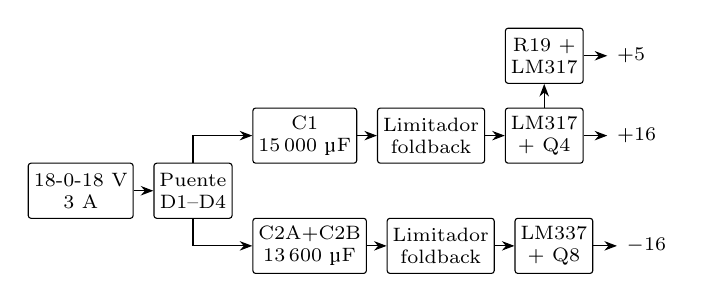
\begin{tikzpicture}[font=\scriptsize, node distance=2.5mm and 2.5mm, b/.style={draw, rounded corners=1pt, align=center, minimum height=7mm, inner sep=2pt}, >={Stealth[length=1.6mm]}]
\node[b] (tr) {18-0-18 V\\3 A};
\node[b, right=of tr] (pt) {Puente\\D1--D4};
\node[b, right=of pt, yshift=7mm] (c1) {C1\\15\,000~µF};
\node[b, right=of pt, yshift=-7mm] (c2) {C2A+C2B\\13\,600~µF};
\node[b, right=of c1] (l1) {Limitador\\foldback};
\node[b, right=of c2] (l2) {Limitador\\foldback};
\node[b, right=of l1] (u1) {LM317\\+ Q4};
\node[b, right=of l2] (u2) {LM337\\+ Q8};
\draw[->] (tr) -- (pt); \draw[->] (pt) |- (c1); \draw[->] (pt) |- (c2);
\draw[->] (c1) -- (l1); \draw[->] (l1) -- (u1); \draw[->] (c2) -- (l2); \draw[->] (l2) -- (u2);
\draw[->] (u1.east) -- ++(3mm,0) node[right]{+16};
\draw[->] (u2.east) -- ++(3mm,0) node[right]{$-$16};
\node[b, above=3mm of u1] (u3) {R19 +\\LM317};
\draw[->] (u1.north) -- (u3.south); \draw[->] (u3.east) -- ++(3mm,0) node[right]{+5};
\end{tikzpicture}
\caption{Diagrama de bloques de la versión 2: estructura de la Fig.~3-1 de~\cite{monografia}, con un limitador con foldback y una ampliación de corriente en cada riel.}
\label{fig:bloques}
\end{figure}

\subsection{Transformador y rectificador}
Cada mitad del secundario da 18~V$_{rms}$. Con la toma central a tierra, el puente D1--D4 (1N5408, 3~A) entrega $+V$ y $-V$ en onda completa, con una caída de diodo por riel ($V_D\approx1{,}1$~V con picos de varios amperios):
\begin{align}
V_p&=18\sqrt{2}-1{,}1=\SI{24,36}{V}\quad\text{(115~V)},\\
V_{p(min)}&=0{,}9\cdot18\sqrt{2}-1{,}1=\SI{21,81}{V},\\
V_{p(max)}&=1{,}21\cdot18\sqrt{2}-1{,}1=\SI{29,7}{V}.
\end{align}
$V_{p(max)}$ incluye la red al $+10$~\% y un 10~\% de subida en vacío. Los capacitores son de 50~V y cada diodo soporta $PIV\approx2V_{p(max)}\approx62$~V, muy por debajo de 1000~V.

Con onda completa, cada mitad del devanado entrega pulsos a un riel en un semiciclo y al otro en el siguiente. Con un riel a 1,67~A y el otro con los PID (0,22~A), la corriente eficaz por mitad es del orden de
\begin{equation}
I_{rms}\approx1{,}6\sqrt{1{,}67^2+0{,}22^2}\approx\SI{2,7}{A}<\SI{3}{A}.
\end{equation}
La simulación da 2,18~A (Sección~\ref{sec:sim}). Si ambos rieles se cargaran a 1,6~A a la vez con la red baja, la corriente subiría a 2,94~A, en el límite del transformador. Por eso la especificación es un riel a la vez.

\subsection{Capacitores de filtro (reutilizados)}
El rizado es de 120~Hz. Con la corriente del filtro (carga más 9~mA del limitador), el rizado y el valle con la red baja son:
\begin{align}
V_{r(pp)+}&=\frac{1{,}683}{120\cdot0{,}015}=\SI{0,94}{V},\quad V_{valle+}=\SI{20,88}{V},\\
V_{r(pp)-}&=\frac{1{,}626}{120\cdot0{,}0136}=\SI{1,00}{V},\quad V_{valle-}=\SI{20,81}{V}.
\end{align}
Con los 50~V nominales de los capacitores y $V_{p(max)}=29{,}7$~V hay margen. El factor de rizado con la red nominal es $F_{r+}=0{,}270/23{,}89=1{,}13$~\% y $F_{r-}=0{,}288/23{,}86=1{,}21$~\%.

\subsection{Caída mínima y margen}
Entre $V_{RAW}$ y la salida hay tres caídas: el limitador ($I R_{SC}+V_{CE}$ del Darlington $\approx0{,}45+1{,}2$~V), la resistencia de la ampliación ($V_{EB}\approx0{,}95$~V) y la caída mínima del LM317 a 0,4~A (2,0~V máximos~\cite{lm317}):
\begin{equation}
V_{RAW(min)}\geq16+0{,}45+1{,}2+0{,}95+2{,}0=\SI{20,6}{V}.
\end{equation}
Con la red al $-10$~\% y 1,67~A, el valle es de 20,88~V. El margen es de 0,27~V con los valores máximos de la hoja de datos, y de unos 0,6~V con los típicos. Es justo, pero la simulación confirma regulación en ese caso (15,97~V). Por eso no conviene ajustar la salida por encima de 16,0~V cuando se prueba con $R_L$ y red baja.

\subsection{Ampliación de corriente (Fig. 3-21)}
Se fija la parte del LM317 en $I_U\approx0{,}39$~A, el 26~\% de su máximo de 1,5~A (la monografía pide menos del 50~\%). El transistor $Q_4$ (TIP42C, 6~A / 65~W~\cite{tip4x}) aporta el resto. Con $h_{FE}\approx30$ a 1,3~A, $I_B=(1{,}674-0{,}39)/30=43$~mA y $V_{EB}\approx0{,}95$~V. Con (\ref{eq:booster}):
\begin{equation}
R_7=\frac{V_{EB}}{I_U-I_B}=\frac{0{,}95}{0{,}39-0{,}043}=\SI{2,74}{\ohm}\rightarrow\SI{2,7}{\ohm},\ 1~\text{W}.
\end{equation}
Con los PID solos (0,27~A), $I_U R_7=0{,}73$~V: la ampliación casi no conduce y el LM317 regula prácticamente solo. En el riel negativo, $Q_8$ (TIP41C) y $R_{15}$ son el espejo. Se agregan $C_9$ y $C_{14}$ ($\SI{220}{\micro F}$) a la salida para los escalones de 1,5~A.

\subsection{Reguladores y red de ajuste}
La red de ajuste es la de la versión 1: $R_1=\SI{120}{\ohm}$ ($R_8$, $R_{16}$, $R_{20}$), con $I_1=10{,}42$~mA, que garantiza la carga mínima de 10~mA y cumple $I_Q\ll I_1\ll I_L$. Para 16~V, por (\ref{eq:vout}), $R_2=(16-1{,}25)/\SI{10,467}{mA}=\SI{1409}{\ohm}$, implementada con $R_9=\SI{1,3}{k\ohm}$ más el trimmer $RV_1=\SI{200}{\ohm}$. El rango de ajuste es de 14,86 a 16,95~V (con la tolerancia de $V_A$, entre 14,27--16,27 y 15,45--17,62~V). Para $+5$~V se usan $R_{21}=\SI{330}{\ohm}$ y $RV_3=\SI{50}{\ohm}$, con rango de 4,70 a 5,23~V. Los capacitores $C_6$, $C_{11}$ y $C_{17}$ de $\SI{10}{\micro F}$ en ADJ elevan el rechazo de rizado a 66--80~dB~\cite{lm317}. Los diodos $D_5$, $D_8$ y $D_{11}$ (OUT$\rightarrow$IN) y $D_6$, $D_9$ y $D_{12}$ (ADJ$\rightarrow$OUT) son las protecciones de la Fig.~3-17 y del Problema~3.6.10.

\subsection{Limitador con foldback}
\label{sec:fb}
\textit{Topología.} Es la Fig.~3-26 (sensor PNP $Q_3$ en paralelo con $R_{SC1}$, que le quita la base al paso PNP) con dos cambios:
\begin{itemize}
\item El transistor de paso es un Darlington ($Q_1$ TIP42C con el driver $Q_2$ BD140~\cite{bd13x}), para que su base necesite solo unos mA.
\item La base de $Q_3$ no va directa al otro lado de $R_{SC1}$, sino a un divisor $R_5$--$R_6$ entre $E_1$ (emisor de $Q_1$) y $V_{A1}$ (salida del limitador). Así se obtiene el foldback de la Fig.~3-27.
\end{itemize}
Con $k'=R_5/(R_5+R_6)$, la tensión base-emisor del sensor es
\begin{equation}
V_{EB3}=I R_{SC1}+k'\,(V_{E1}-V_{A1}).
\label{eq:veb3}
\end{equation}
En operación normal $Q_1$ está saturado, $V_{E1}-V_{A1}\approx1{,}2$~V, y el término de foldback es casi nulo y no depende de la red. En un cortocircuito, $V_{A1}$ cae a la caída mínima del regulador ($\approx2{,}9$~V), $V_{E1}-V_{A1}$ sube a unos 20~V y la corriente necesaria para activar el sensor baja. Es la misma idea de las ecs.~(3.29)--(3.35), con la tensión de referencia tomada sobre el transistor de paso.

\textit{Cálculo.} Se elige $R_{SC1}=\SI{0,27}{\ohm}$ (5~W) y $k'=270/(270+12\,000)=0{,}022$ ($R_5=\SI{270}{\ohm}$, $R_6=\SI{12}{k\ohm}$). Con $V_{BE}=0{,}7$~V:
\begin{align}
I_{lim}&=\frac{0{,}7-0{,}022\cdot1{,}2}{0{,}27}=\SI{2,49}{A}\quad\text{(sobrecarga)},\\
I_{SC}&=\frac{0{,}7-0{,}022\,(V_{E1}-V_{A1})}{0{,}27}.
\end{align}
Con $V_{E1}-V_{A1}=20{,}5$~V (red nominal), $I_{SC}=0{,}91$~A. Con la red baja es de 1,11~A y con la red alta de 0,70~A. El transistor de paso disipa entonces 18,8, 20,2 y 16,2~W, frente a unos 45~W sin foldback.

\textit{Arranque con $R_L$ conectada.} Un foldback demasiado fuerte puede dejar la salida trabada al encender con carga: si en algún punto de la subida el límite fuera menor que lo que pide $R_L$, la tensión no seguiría subiendo. La condición es que el límite supere la demanda para toda tensión $x$ entre 0 y 16~V:
\begin{equation}
\frac{V_{BE}-k'\,(V_{E1}-x-2{,}9)}{R_{SC}}>\frac{x}{R_L}+I_{int}.
\end{equation}
Se evaluó en el peor caso (red al $+10$~\%, que da más foldback, y $V_{BE}=0{,}65$~V). El margen mínimo es de 0,16~A. Con $R_5=\SI{330}{\ohm}$ el margen caía a 0,03~A, y por eso se eligió \SI{270}{\ohm}. La simulación confirma el arranque con $R_L$ en los dos extremos de red (Fig.~\ref{fig:sim_arr}).

\textit{Polarización.} El Darlington necesita $I_B\geq2{,}5/(15\cdot40)=4{,}2$~mA para conducir el límite con las ganancias mínimas. Con $R_3=\SI{2,7}{k\ohm}$ a tierra, $I_B=(20{,}88-0{,}45-1{,}6)/2700=7{,}0$~mA, que permite hasta 4,2~A. $R_3$ disipa como máximo $29{,}7^2/2700=0{,}33$~W, y se usa de 1~W. $R_4=\SI{1}{k\ohm}$ entre base y emisor de $Q_1$ drena las corrientes de fuga del driver. $Q_3$ (BC557~\cite{bc547}) solo tiene que desviar la corriente de $R_3$, unos 11~mA como máximo. El riel negativo usa $Q_5$ (TIP41C), $Q_6$ (BD139), $Q_7$ (BC547) y $R_{11}$--$R_{14}$.

\subsection{Rama de +5~V}
No cambia respecto a la versión 1. $U_3$ (LM317) se alimenta desde $+16$~V por $R_{19}=\SI{100}{\ohm}/3$~W. $V_{IN3}=16-0{,}057\cdot100=10{,}3$~V, de modo que regula hasta 91~mA. En un corto, $R_{19}$ fija la corriente en $(16-1{,}5)/100=145$~mA. El filtro $R_{19}C_{15}$ tiene un corte de 15,9~Hz y atenúa 11,8~dB adicionales a 60~Hz.

\subsection{Disipación y disipadores}
Cada riel lleva un disipador en el borde de la placa con sus cuatro semiconductores de potencia ($Q_1$, $Q_2$, $Q_4$ y U1 en el superior), todos con mica y buje, porque cada aleta está unida a un pin. La Tabla~\ref{tab:pot} resume la potencia. Se usan $\theta_{JC}=1{,}92$~°C/W para los TIP4xC, 5~°C/W para el LM317, $\theta_{CS}=1$~°C/W para mica con grasa y $T_A=40$~°C.

\begin{table}[htbp]
\caption{Potencia en el riel +16~V (red nominal / red +10~\%)}
\label{tab:pot}
\centering
\footnotesize
\begin{tabular}{@{}lcc@{}}
\toprule
Elemento & Con $R_L$ (1,67~A) & Corto (foldback) \\
\midrule
Q1+Q2 (Darlington) & 2,0 / 2,0~W & 18,8 / 16,2~W \\
Q4 (ampliación) & 8,0 / 11,2~W & $\approx$0 \\
U1 LM317 & 2,1 / 3,1~W & $<$1~W \\
Total en el disipador & 12,1 / 16,3~W & $\leq$20,2~W (red baja) \\
\bottomrule
\end{tabular}
\end{table}

Con un disipador de $\theta_{SA}=2$~°C/W:
\begin{itemize}
\item Con $R_L$ y red alta, el disipador queda a $40+16{,}3\cdot2=73$~°C. Las junturas: $Q_4$ a $73+11{,}2\cdot2{,}92=106$~°C y U1 a $73+3{,}1\cdot6=92$~°C.
\item En corto con red baja, el disipador llega a $40+20{,}2\cdot2=80$~°C y $Q_1$ a $80+20{,}2\cdot2{,}92=139$~°C, por debajo de 150~°C.
\end{itemize}
Por tanto se pide \textbf{un disipador de $\leq2$~°C/W por riel}, por ejemplo un perfil aletado de unos $100\times60\times30$~mm. $U_3$ (+5~V) no necesita disipador.

\subsection{Protecciones}
\begin{itemize}
\item \textbf{F1} (T1~A, lento) en el primario. El transformador es de 108~VA y el consumo estimado es de 0,53~A.
\item \textbf{F2 y F3} (T3,15~A, lentos), uno en cada mitad del secundario.
\item \textbf{Limitadores con foldback} en $\pm16$~V: 2,4~A en sobrecarga y 0,7--1,2~A en corto, sostenible indefinidamente con recuperación automática.
\item \textbf{$R_{19}$} limita $+5$~V a 0,145~A. Un corto en $+5$~V no apaga los $\pm16$~V.
\item \textbf{Protección térmica interna} de LM317/LM337 como respaldo, y \textbf{diodos} OUT$\rightarrow$IN y ADJ$\rightarrow$OUT.
\item \textbf{Diodos de polaridad inversa} $D_7$ y $D_{10}$ (1N5408~\cite{d1n5408}, por la corriente de 2,4~A si se cruzan los rieles) y $D_{13}$.
\item \textbf{Tierra en un solo punto}: la fuente no une GND con PGND.
\item \textbf{Carga de prueba removible}: $R_L$ va en las borneras J4/J5, fuera de la placa, porque disipa 26~W.
\end{itemize}

% =========================================================
\section{Esquemáticos}
% =========================================================
Las Figs.~\ref{fig:esq_entrada} a \ref{fig:esq_salida} muestran cada etapa con referencias y valores. La numeración es la misma del archivo EAGLE, de la placa y de la lista de materiales. El esquemático completo está en el Apéndice (Fig.~\ref{fig:completo}).

\begin{figure*}[!t]
\centering
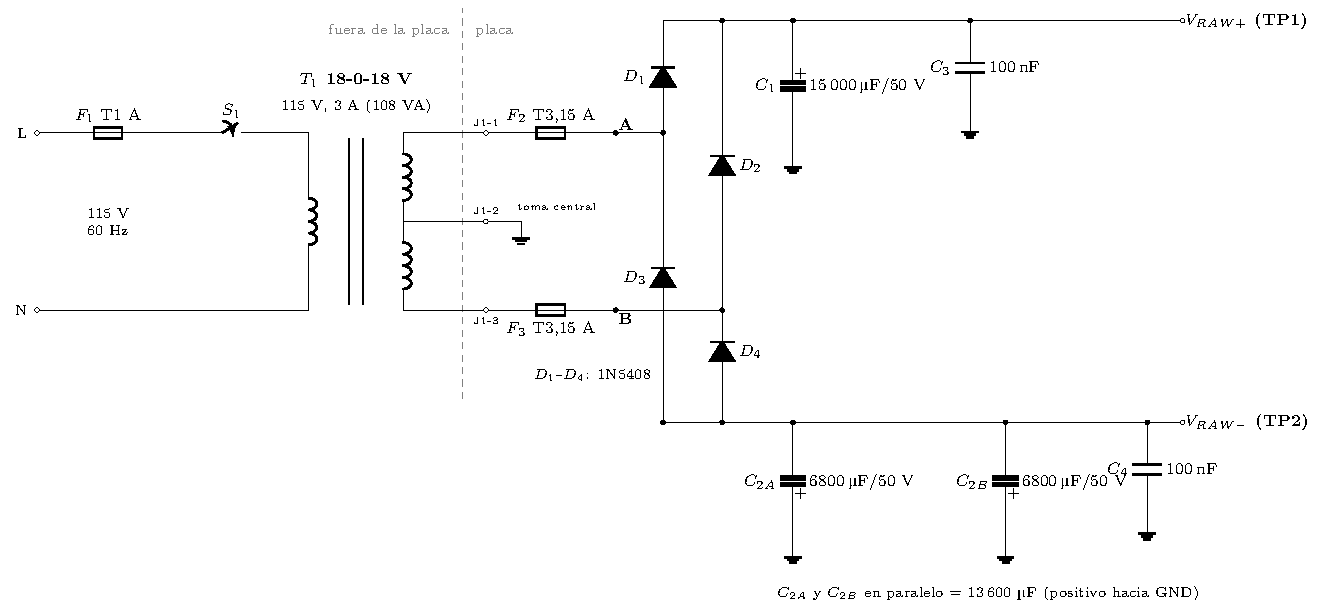
\includegraphics[width=0.86\textwidth]{esq_entrada.pdf}
\caption{Etapa 1: red, F1 y S1 (fuera de la placa), transformador 18-0-18~V / 3~A, bornera J1, fusibles F2 y F3, puente D1--D4 y filtros C1 ($+$) y C2A+C2B ($-$).}
\label{fig:esq_entrada}
\end{figure*}

\begin{figure*}[!t]
\centering
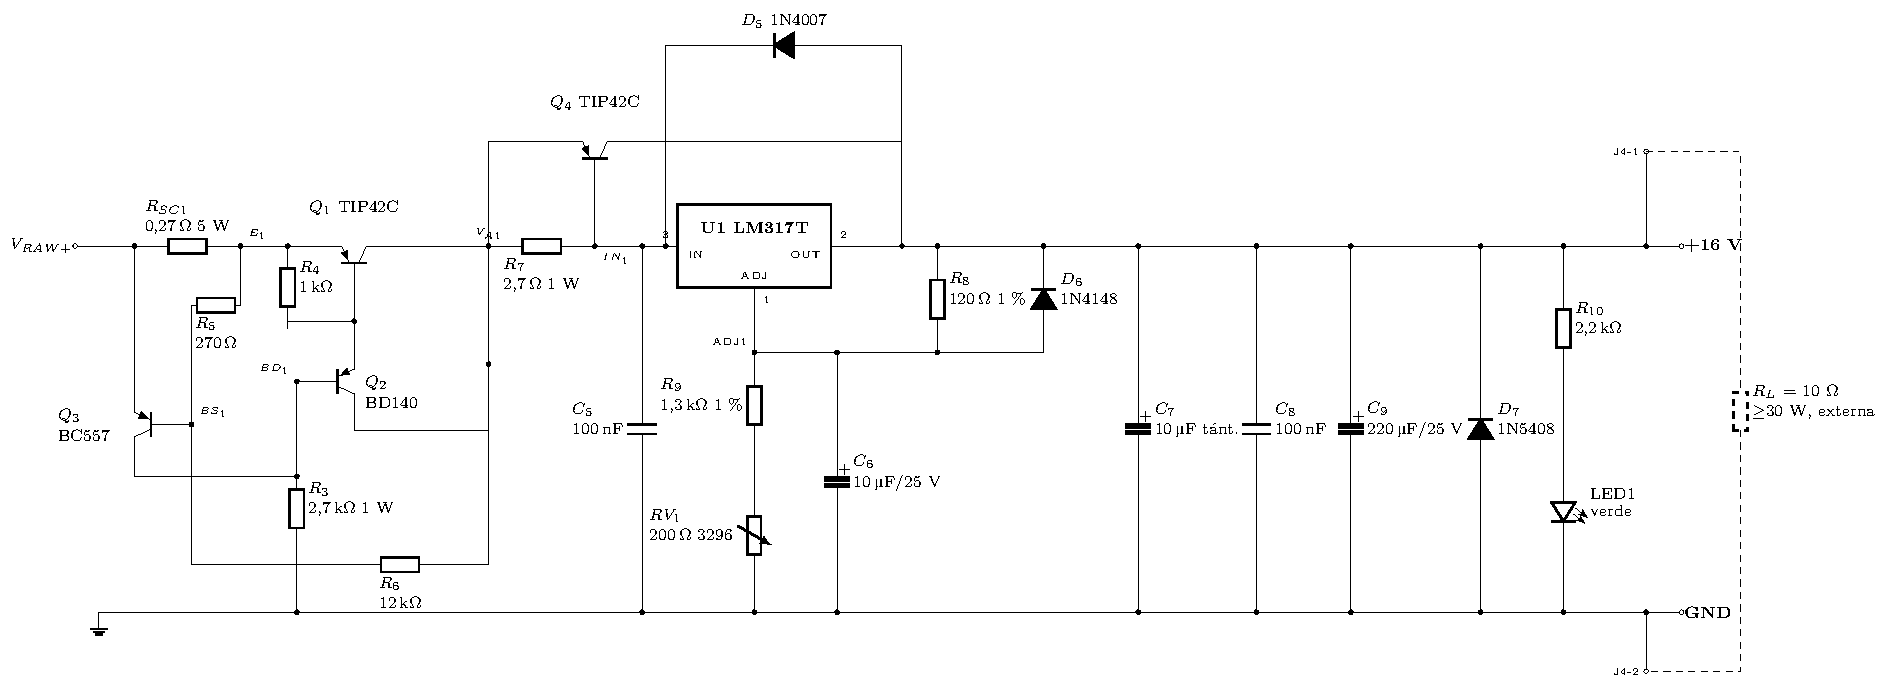
\includegraphics[width=\textwidth]{esq_pos.pdf}
\caption{Etapa 2: riel de +16~V. Limitador con foldback ($R_{SC1}$, Darlington $Q_1$--$Q_2$, sensor $Q_3$, divisor $R_5$--$R_6$), ampliación de corriente ($R_7$, $Q_4$, Fig.~3-21), regulador U1 y salida con la bornera J4 para la carga de prueba removible $R_L$.}
\label{fig:esq_pos}
\end{figure*}

\begin{figure*}[!t]
\centering
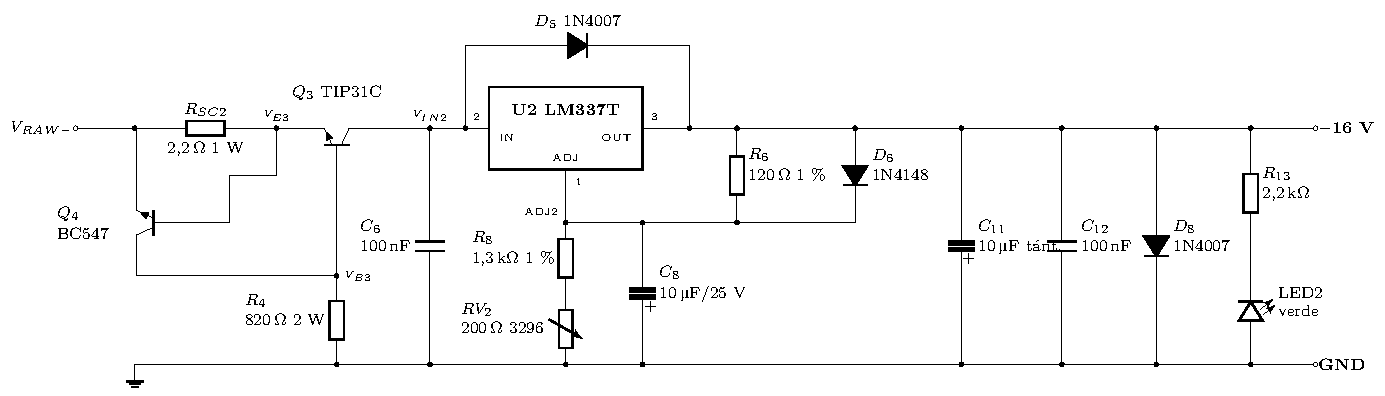
\includegraphics[width=\textwidth]{esq_neg.pdf}
\caption{Etapa 3: riel de $-16$~V, espejo de la etapa 2 con $Q_5$ TIP41C, $Q_6$ BD139, $Q_7$ BC547, $Q_8$ TIP41C, U2 LM337 y la bornera J5.}
\label{fig:esq_neg}
\end{figure*}

\begin{figure*}[!t]
\centering
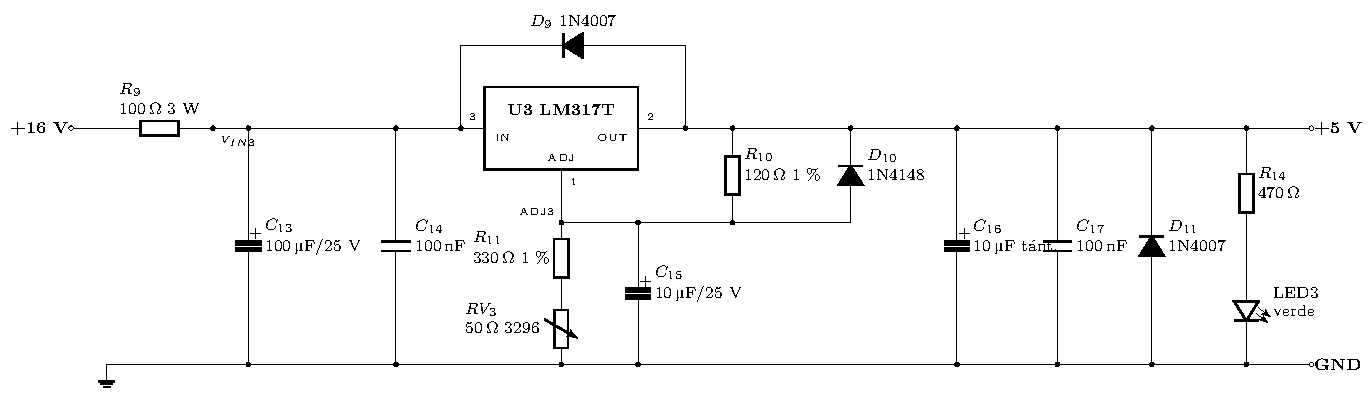
\includegraphics[width=0.86\textwidth]{esq_5v.pdf}
\caption{Etapa 4: riel de +5~V tomado de +16~V por $R_{19}$, con el regulador U3 LM317.}
\label{fig:esq_5v}
\end{figure*}

\begin{figure}[htbp]
\centering
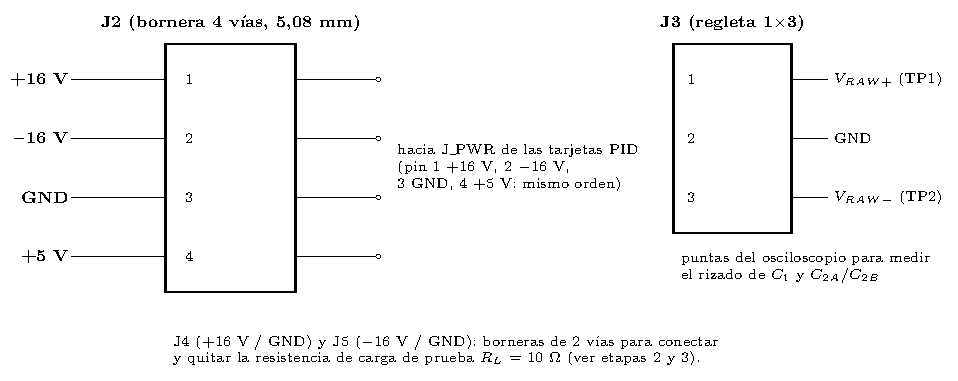
\includegraphics[width=\linewidth]{esq_salida.pdf}
\caption{Bornera de salida J2 (hacia \texttt{J\_PWR} de las tarjetas PID), regleta de prueba J3 y borneras J4/J5 de la carga.}
\label{fig:esq_salida}
\end{figure}

% =========================================================
\section{Simulación}
\label{sec:sim}
% =========================================================
\subsection{Método}
Se simuló el circuito completo en ngspice~42~\cite{ngspice} con análisis transitorio. Los diodos y los BC547/BC557 usan parámetros publicados. El LM317 y el LM337 son \emph{modelos de comportamiento} propios: reproducen la referencia de 1,25~V, $I_Q$, la caída mínima, la regulación de línea de 0,01~\%/V y el límite interno de 1,5~A. Los TIP41C/TIP42C y BD139/BD140 usan modelos genéricos con $h_{FE}\approx50$ y 80. El transformador es una fuente por mitad de 19,4~V$_{rms}$ en vacío, con \SI{0,45}{\ohm} y 0,3~mH. $R_L$ y los PID se modelan como conductancias que se conectan y desconectan en el tiempo, igual que en la prueba real. Los promedios se calculan con muestreo uniforme. Los archivos están en \texttt{fuente/simulacion/}.

\subsection{Resultados}
La Tabla~\ref{tab:sim} compara cálculo y simulación.

\begin{table}[htbp]
\caption{Cálculo frente a simulación}
\label{tab:sim}
\centering
\scriptsize\setlength{\tabcolsep}{3pt}
\resizebox{\linewidth}{!}{\begin{tabular}{@{}lcc@{}}
\toprule
Magnitud & Cálculo & Simulación \\
\midrule
$V_{RAW+}$ media / rizado ($R_L$, 115~V) & 23,9~V / 0,94~V$_{pp}$ & 22,8~V / 0,60~V$_{pp}$ \\
+16~V sin / con $R_L$ & 16,00 / $\geq$15,92~V & 15,991 / 15,977~V \\
$-16$~V sin / con $R_L$ & $-16{,}00$ / $\leq-15{,}92$~V & $-15{,}993$ / $-15{,}978$~V \\
Corriente en $R_L$ & 1,60~A & 1,598~A \\
Corriente de $Q_4$ / del LM317 & 1,28 / 0,39~A & 1,33 / 0,26~A \\
\%Reg (\ref{eq:reg}) +16 / $-16$ / +5 & $\leq$0,5~\% & 0,09 / 0,10 / 0,00~\% \\
Rizado de salida $\pm16$~V con $R_L$ & $<$0,4~mV$_{pp}$ & 0,11 / 0,12~mV$_{pp}$ \\
$\Delta V_{out}$ por línea $\pm10$~\% & $\leq$33~mV & 8,8~mV \\
+16~V, red $-10$~\% y $R_L$ & regula & 15,974~V \\
$I_{rms}$ por mitad del secundario & $\approx$2,7~A & 2,18~A \\
Límite en sobrecarga & 2,49~A & 2,35--2,38~A \\
$I$ de corto +16 / $-16$ / +5 & 0,91 / 0,91 / 0,145~A & 0,84 / 0,90 / 0,14~A \\
$P$ del Darlington en corto & 18,8~W & 17,8 / 18,9~W \\
Recuperación tras el corto con $R_L$ & 16~V & 15,98~V \\
Arranque con $R_L$, red $\pm10$~\% & sin trabarse & 15,97 / 15,98~V \\
\bottomrule
\end{tabular}}
\end{table}

\begin{figure}[htbp]
\centering
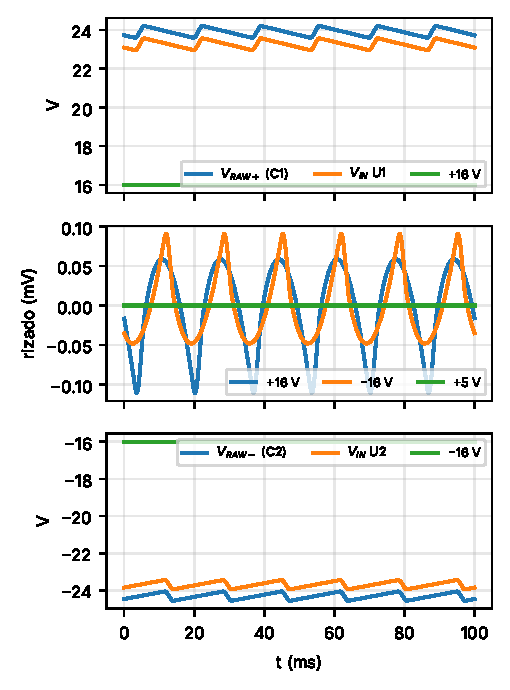
\includegraphics[width=\linewidth]{sim_regimen.pdf}
\caption{Régimen con $R_L$ en +16~V (1,6~A) y red nominal: tensiones del riel, rizado de salida y reparto de corriente entre la ampliación $Q_4$ y el LM317.}
\label{fig:sim_reg}
\end{figure}

\begin{figure}[htbp]
\centering
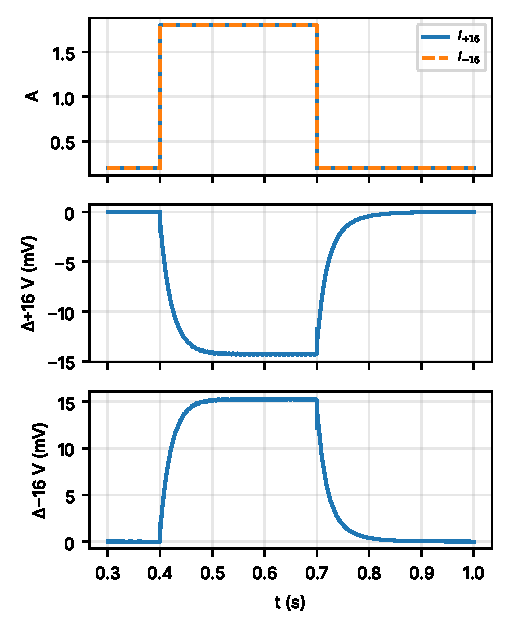
\includegraphics[width=\linewidth]{sim_carga.pdf}
\caption{Conexión de $R_L$ en $t=0{,}4$~s y desconexión en $t=0{,}7$~s en los dos rieles (los PID siempre conectados): corrientes y desviación de cada salida.}
\label{fig:sim_carga}
\end{figure}

\begin{figure}[htbp]
\centering
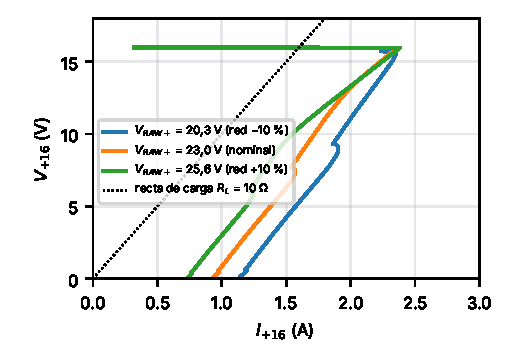
\includegraphics[width=\linewidth]{sim_foldback.pdf}
\caption{Curva V--I del riel +16~V con foldback (Fig.~3-27b de la monografía), para tres tensiones de entrada. La recta de $R_L=\SI{10}{\ohm}$ no corta la rama de foldback: la fuente no se traba con la carga de prueba.}
\label{fig:sim_fb}
\end{figure}

\begin{figure}[htbp]
\centering
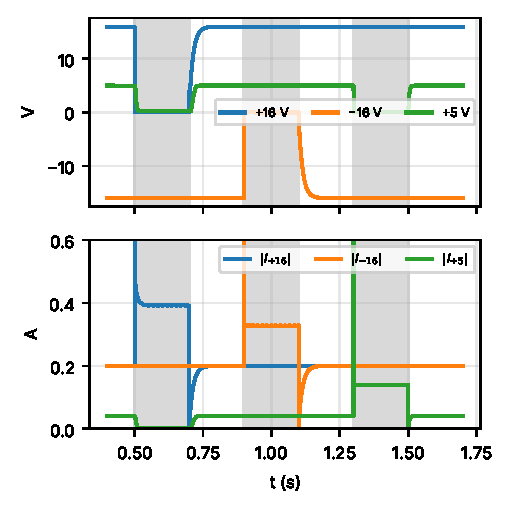
\includegraphics[width=\linewidth]{sim_corto.pdf}
\caption{Cortocircuitos sucesivos (zonas grises) de +16~V, $-16$~V y +5~V con $R_L$ conectada en los dos rieles. El pico inicial es la descarga de los capacitores de salida. Al quitar cada corto, la salida vuelve a su valor con la carga puesta.}
\label{fig:sim_corto}
\end{figure}

\begin{figure}[htbp]
\centering
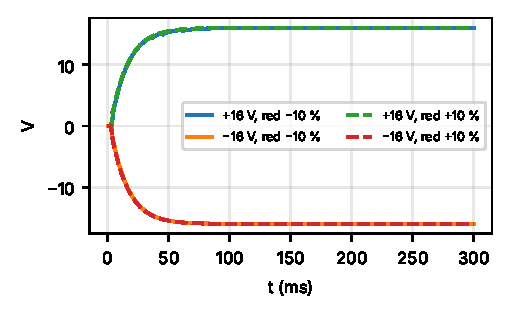
\includegraphics[width=\linewidth]{sim_arranque.pdf}
\caption{Arranque desde cero con $R_L$ conectada en ambos rieles, con la red al $-10$~\% y al $+10$~\%.}
\label{fig:sim_arr}
\end{figure}

\subsection{Análisis}
\textit{Filtro.} El rizado simulado es menor que el calculado (0,60 frente a 0,94~V$_{pp}$), porque el cálculo supone descarga durante todo el semiperiodo. La tensión media es 1~V menor, por la resistencia del devanado y la caída real de los diodos con picos de varios amperios. Aun así, con la red al $-10$~\% el regulador sigue regulando (15,974~V).

\textit{Reparto de corriente.} Con $R_L$, $Q_4$ lleva 1,33~A y el LM317 solo 0,26~A, el 17~\% de su máximo, por debajo del 50~\% que recomienda la monografía. Por eso el integrado disipa unos 2~W y no hacía falta cambiarlo.

\textit{Regulación.} Conectar y quitar $R_L$ cambia la salida 14~mV en régimen (0,09~\%), con transitorios de 13~mV que se recuperan en unos 20~ms (Fig.~\ref{fig:sim_carga}). La regulación de línea es de 8,8~mV para $\pm10$~\% de red y el rizado de salida es de 0,1~mV$_{pp}$. En $+5$~V, las dos etapas en cascada y el filtro $R_{19}C_{15}$ dejan un rizado despreciable.

\textit{Foldback.} La curva V--I (Fig.~\ref{fig:sim_fb}) tiene la forma de la Fig.~3-27b. La salida se mantiene en 16~V hasta unos 2,35~A y luego la corriente se pliega hasta 0,8--1,2~A en corto, menos cuanto mayor es la tensión de red, como predice (\ref{eq:veb3}). El límite simulado (2,35~A) es algo menor que el calculado (2,49~A), porque el BC557 empieza a conducir con unos 0,66~V. La recta de $R_L$ queda siempre a la izquierda de la rama de foldback, así que la carga de prueba no traba la fuente. Lo confirman el arranque con red alta y baja (Fig.~\ref{fig:sim_arr}) y la recuperación después de cada corto con $R_L$ puesta (Fig.~\ref{fig:sim_corto}).

\textit{Cortocircuito.} En corto, el Darlington disipa 17,8~W (+16~V) y 18,9~W ($-16$~V), y ese valor define el disipador de 2~°C/W. Un corto en $+5$~V no afecta a $+16$~V (15,98~V).

% =========================================================
\section{Circuito impreso}
% =========================================================
La placa es de una sola cara, de $190{,}5\times139{,}7$~mm, para una baquela de $20\times15$~cm (Figs.~\ref{fig:pcb_ens} y \ref{fig:pcb_cu}). Se generó con un programa propio en Python, el mismo usado para las tarjetas PID~\cite{informepid}: colocación por recocido simulado dentro de regiones por etapa y ruteo negociado. Las reglas de diseño son:
\begin{itemize}
\item Pistas de 0,8~mm, y de 1,6~mm para las redes de corriente alta: secundario, $V_{RAW\pm}$, emisores y colectores de los transistores de paso, salidas $\pm16$~V y GND. Con cobre de 35~µm, 1,6~mm conducen unos 3~A con 10~°C de aumento.
\item Pads de 2,0~mm, y de 2,6~mm en borneras, portafusibles, diodos 1N5408, $R_{SC}$ y capacitores grandes.
\item Separación mínima entre redes de 0,40~mm, verificada sobre la geometría final.
\end{itemize}
Las 32 redes quedan completas, sin cortos, y el esquemático y la placa son consistentes. Hay siete puentes de alambre del lado de componentes (P1--P7, lista en \texttt{puentes.md}), todos en redes de señal o de baja corriente.

Los cuatro semiconductores de potencia de cada riel van alineados en un borde con la aleta hacia afuera: $Q_1$, $Q_2$, $Q_4$ y U1 arriba, y $Q_5$, $Q_6$, $Q_8$ y U2 abajo. Así se atornillan a un solo disipador por riel. Los capacitores de filtro están en el borde izquierdo y las borneras de salida (J2, J4, J5) en el derecho. En las esquinas hay cuatro agujeros de montaje de 3,2~mm.

En la carpeta \texttt{fuente/hardware/pcb/} están:
\begin{itemize}
\item \texttt{fuente.sch} y \texttt{fuente.brd}, en formato EAGLE, que Fusion Electronics abre.
\item \texttt{cobre\_espejado\_1a1.pdf}: el cobre espejado a escala 1:1, con una regla de 50~mm para comprobar la escala.
\item \texttt{ensamble\_1a1.pdf}: vista de componentes a 1:1 y una vista ampliada con valores.
\item \texttt{puentes.md}: la lista de los siete puentes.
\end{itemize}

\begin{figure*}[!t]
\centering
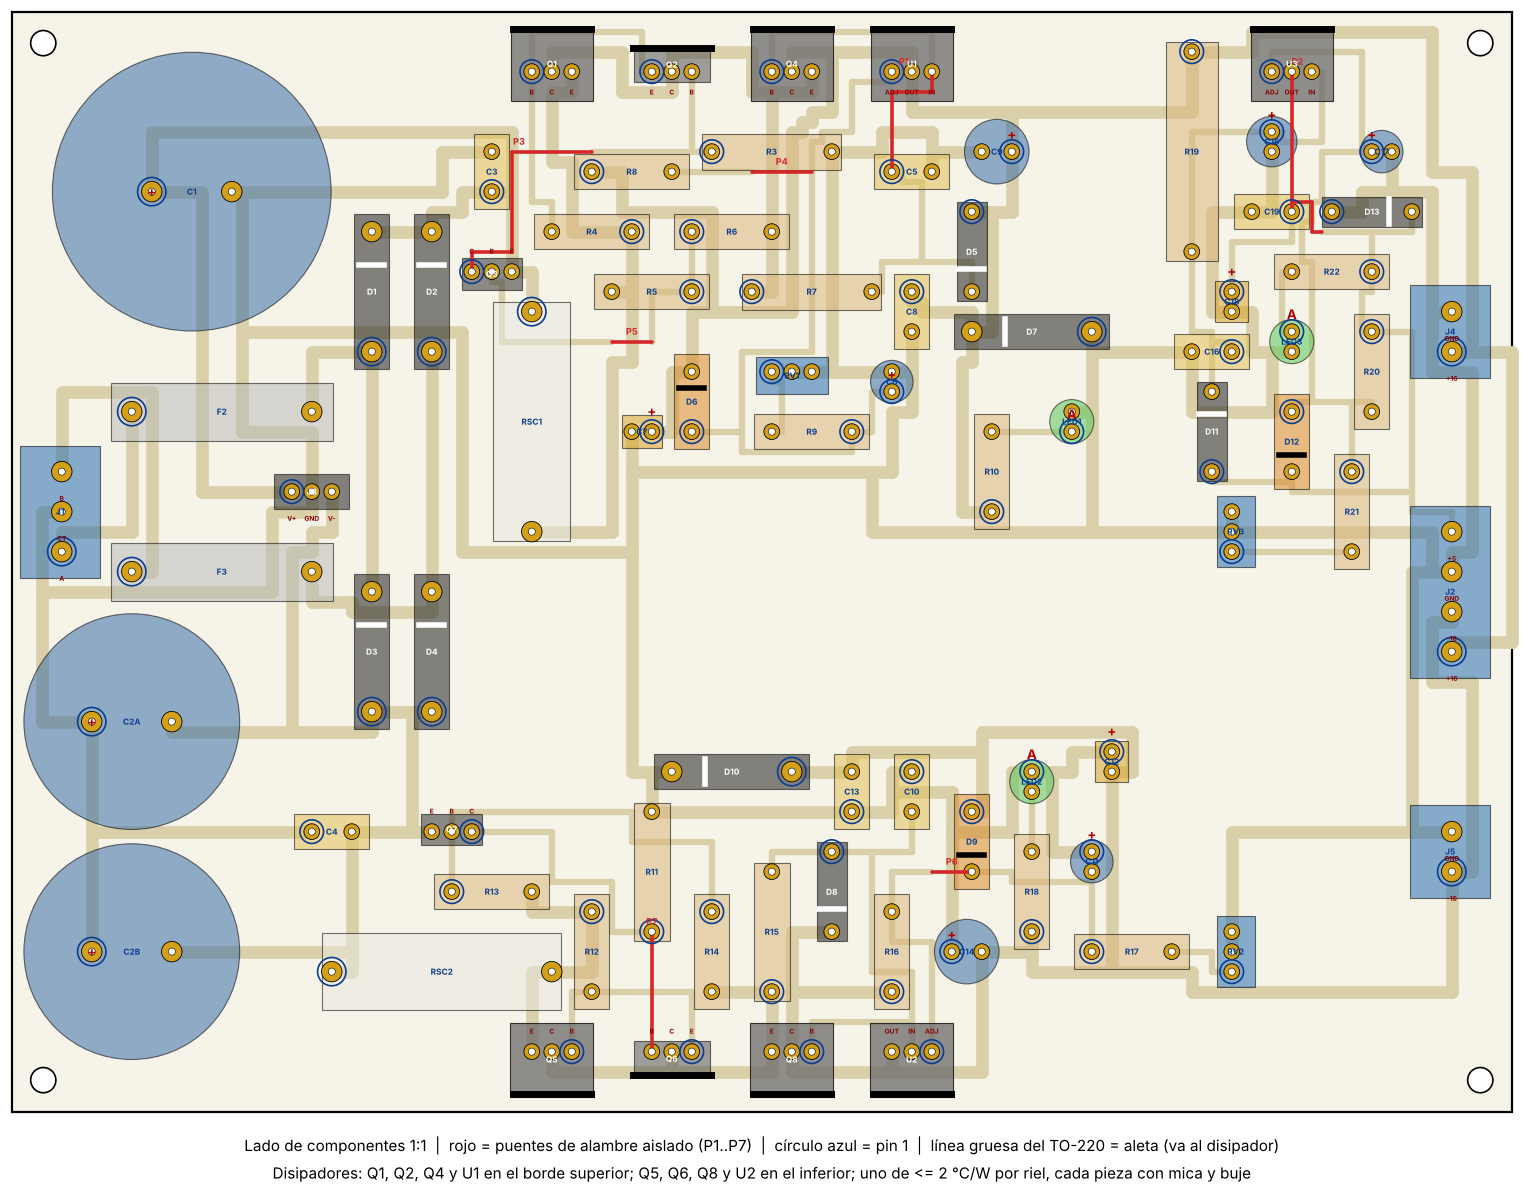
\includegraphics[width=0.9\textwidth]{pcb_ensamble.png}
\caption{Vista de ensamble (lado de componentes). Rojo: puentes de alambre P1--P7. Línea gruesa de cada TO-220/TO-126: aleta, que va al disipador. Círculo azul: pin~1.}
\label{fig:pcb_ens}
\end{figure*}

\begin{figure}[htbp]
\centering
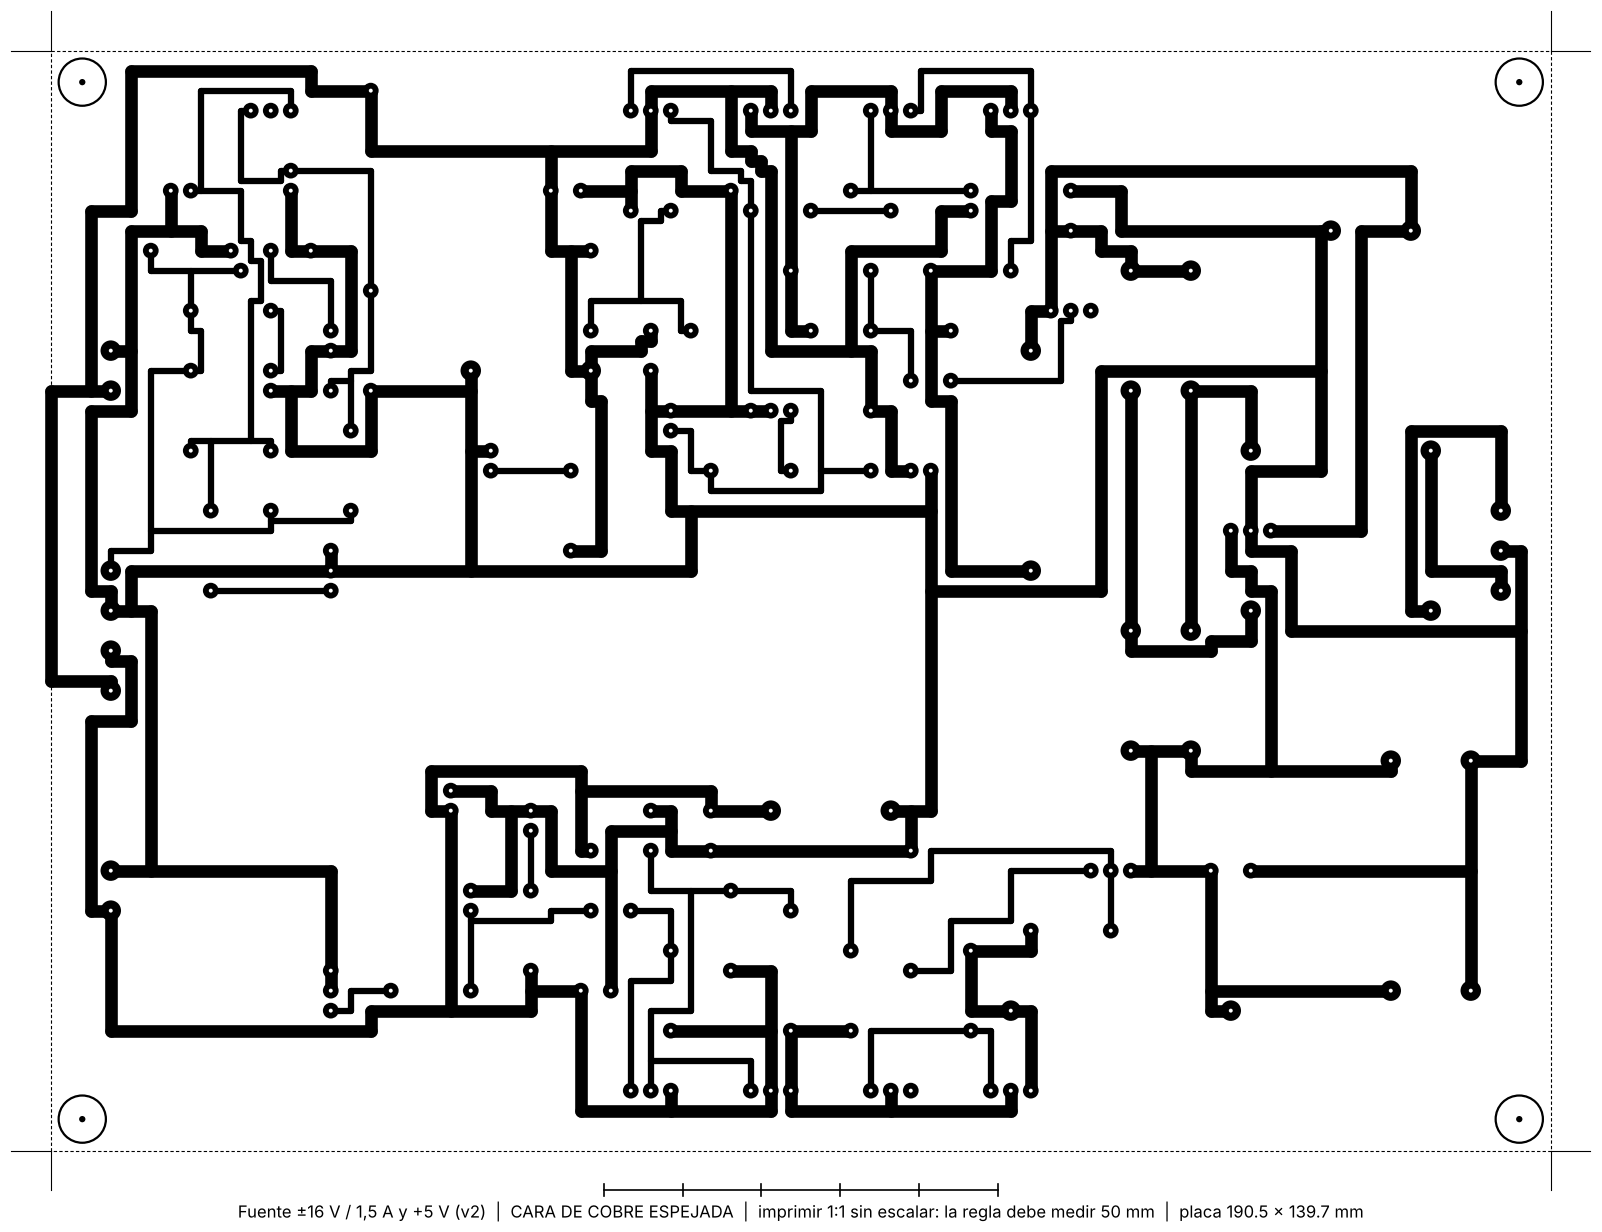
\includegraphics[width=\linewidth]{pcb_cobre_espejado.png}
\caption{Cara de cobre espejada (reducida; la hoja para imprimir es la de 1:1).}
\label{fig:pcb_cu}
\end{figure}

\subsection{Guía de conexión}
La Tabla~\ref{tab:conex} indica cómo se conecta la fuente. Las salidas de J2 llevan el mismo orden que \texttt{J\_PWR} de las tarjetas PID, así que basta un cable de cuatro hilos a una tarjeta, y de ella a la otra. La carga de prueba $R_L$ se atornilla en J4 o J5 solo durante la prueba de 1,5~A, y se retira para medir sin carga o para alimentar los PID. La fuente de las bobinas va por separado a \texttt{J\_VBOB}, y GND con PGND se unen solo en un \texttt{JP\_GND}.

\begin{table}[htbp]
\caption{Guía de conexión}
\label{tab:conex}
\centering
\footnotesize
\begin{tabular}{@{}p{0.42\linewidth}p{0.48\linewidth}@{}}
\toprule
Desde & Hacia \\
\midrule
Red L $\rightarrow$ F1 T1~A $\rightarrow$ S1 & Primario del transformador \\
Red N & Otro extremo del primario \\
Secundario: extremo A / toma central / extremo B & J1-1 / J1-2 (GND) / J1-3 \\
J2-1/2/3/4 (+16, $-16$, GND, +5) & \texttt{J\_PWR} 1/2/3/4 de la tarjeta PID A; de A a B por su \texttt{J\_PWR} \\
J4-1 (+16) y J4-2 (GND) & $R_L=\SI{10}{\ohm}$, $\geq$30~W, removible \\
J5-1 ($-16$) y J5-2 (GND) & $R_L$, removible (un riel a la vez) \\
J3 ($V_{RAW+}$, GND, $V_{RAW-}$) & Osciloscopio (rizado) \\
Disipador superior ($\leq$2~°C/W) & $Q_1$, $Q_2$, $Q_4$ y U1, con mica y buje \\
Disipador inferior ($\leq$2~°C/W) & $Q_5$, $Q_6$, $Q_8$ y U2, con mica y buje \\
\bottomrule
\end{tabular}
\end{table}


% =========================================================
\section{Lista de materiales}
% =========================================================
La Tabla~\ref{tab:bom} es la lista de materiales; la versión con sustitutos está en \texttt{fuente/hardware/lista\_de\_materiales.csv}. El LM317, el LM337 y los capacitores de $\SI{15000}{\micro F}$ y $\SI{6800}{\micro F}$ ya estaban disponibles; el transformador hay que comprarlo.

\begin{table}[htbp]
\caption{Lista de materiales}
\label{tab:bom}
\centering
\scriptsize\setlength{\tabcolsep}{3pt}
\begin{tabular}{@{}p{0.33\linewidth}p{0.50\linewidth}c@{}}
\toprule
Referencia & Componente & Cant. \\
\midrule
T1 & Transformador 18-0-18~V / 3~A, 115~V & 1 \\
F1 / F2, F3 & Fusible 5$\times$20 lento T1~A / T3,15~A, con portafusibles & 1 / 2 \\
S1 & Interruptor 250~VAC & 1 \\
D1--D4, D7, D10 & 1N5408 & 6 \\
D5, D8, D11, D13 / D6, D9, D12 & 1N4007 / 1N4148 & 4 / 3 \\
C1 / C2A, C2B & $\SI{15000}{\micro F}$ / $\SI{6800}{\micro F}$, 50~V (disponibles) & 1 / 2 \\
C3, C4, C5, C8, C10, C13, C16, C19 & 100~nF cerámico & 8 \\
C6, C11, C17 / C7, C12, C18 & $\SI{10}{\micro F}$ electrolítico / tántalo & 3 / 3 \\
C9, C14 / C15 & $\SI{220}{\micro F}$ / $\SI{100}{\micro F}$, 25~V & 2 / 1 \\
$R_{SC1}$, $R_{SC2}$ & $\SI{0,27}{\ohm}$, 5~W & 2 \\
R3, R11 / R7, R15 & $\SI{2,7}{k\ohm}$ / $\SI{2,7}{\ohm}$, 1~W & 2 / 2 \\
R4, R12 / R5, R13 / R6, R14 & $\SI{1}{k\ohm}$ / $\SI{270}{\ohm}$ / $\SI{12}{k\ohm}$ & 2 / 2 / 2 \\
R8, R16, R20 / R9, R17 / R21 & $\SI{120}{\ohm}$ / $\SI{1,3}{k\ohm}$ / $\SI{330}{\ohm}$, 1~\% & 3 / 2 / 1 \\
R19 & $\SI{100}{\ohm}$, 3~W & 1 \\
R10, R18 / R22 & $\SI{2,2}{k\ohm}$ / $\SI{470}{\ohm}$ & 2 / 1 \\
RV1, RV2 / RV3 & Trimmer 3296W $\SI{200}{\ohm}$ / $\SI{50}{\ohm}$ & 2 / 1 \\
Q1, Q4 / Q5, Q8 & TIP42C / TIP41C & 2 / 2 \\
Q2 / Q6 & BD140 / BD139 & 1 / 1 \\
Q3 / Q7 & BC557 / BC547 & 1 / 1 \\
U1, U3 / U2 & LM317T / LM337T (disponibles) & 2 / 1 \\
LED1--LED3 & LED verde 5~mm & 3 \\
J1 / J2 / J3 / J4, J5 & Bornera 3 vías / 4 vías / regleta 1$\times$3 / bornera 2 vías & 1/1/1/2 \\
$R_L$ (externa) & $\SI{10}{\ohm}$, $\geq$30~W & 1 \\
-- & Disipador $\leq$2~°C/W (3 TO-220 + 1 TO-126) & 2 \\
-- & Mica, buje y tornillo M3 & 8 \\
-- & Baquela una cara 20$\times$15~cm & 1 \\
\bottomrule
\end{tabular}
\end{table}

% =========================================================
\section{Plan de pruebas}
% =========================================================
Las pruebas van de menor a mayor riesgo. El detalle está en \texttt{fuente/pruebas/plan\_de\_pruebas.md}.
\begin{enumerate}
\item[P0] \textit{Sin energía:} polaridades, ausencia de cortos y aislamiento aleta--disipador.
\item[P1] \textit{Primer encendido} sin carga: V~AC por mitad, $V_{RAW\pm}$ y LED.
\item[P2] \textit{Ajuste} con $RV_1$--$RV_3$ y rango de cada trimmer.
\item[P3] \textit{1,5~A y regulación de carga} con (\ref{eq:reg}): medir sin $R_L$, atornillar $R_L$ en J4 (o J5), medir tensión y corriente y volver a quitarla.
\item[P4] \textit{Rizado} sobre los filtros (120~Hz) y en las salidas, con $R_L$.
\item[P5] \textit{Regulación de línea} con variac, si se dispone de uno.
\item[P6] \textit{Cortocircuito y foldback}, con y sin $R_L$, en cada riel, con recuperación y temperatura tras 60~s.
\item[P7] \textit{Curva V--I} con carga variable.
\item[P8] \textit{Arranque con $R_L$} cinco veces.
\item[P9] \textit{Temperatura} tras 30~min con $R_L$.
\item[P10] \textit{Tarjetas PID} sin $R_L$ y sin bobinas.
\end{enumerate}
La Tabla~\ref{tab:med} es la tabla para llenar. La versión completa, de 40 filas, está en \texttt{mediciones.csv}.

\begin{table}[htbp]
\caption{Tabla de mediciones prácticas (para llenar)}
\label{tab:med}
\centering
\scriptsize\setlength{\tabcolsep}{3pt}
\begin{tabular}{@{}p{0.08\linewidth}p{0.36\linewidth}p{0.24\linewidth}p{0.11\linewidth}p{0.07\linewidth}@{}}
\toprule
Prueba & Magnitud & Esperado & Medido & Error \\
\midrule
P1 & V~AC por mitad del secundario & 18--20~V$_{rms}$ & & \\
P2 & Rango de $RV_1$ / $RV_2$ & $\pm$14,9 a $\pm$17,0~V & & \\
P3 & +16~V sin / con $R_L$ & 16,00 / $\geq$15,92~V & & \\
P3 & Corriente en $R_L$ (+16) & $\geq$1,5~A (1,6~A) & & \\
P3 & $-16$~V sin / con $R_L$ & $-16{,}00$ / $\leq-15{,}92$~V & & \\
P3 & Corriente en $R_L$ ($-16$) & $\geq$1,5~A (1,6~A) & & \\
P3 & \%Reg +16 / $-16$ & $\leq$0,5~\% & & \\
P4 & Rizado sobre C1 / C2 & 0,6--0,9 / 0,65--1,0~V$_{pp}$ & & \\
P4 & Rizado de salida $\pm16$~V & $<$1~mV$_{pp}$ & & \\
P5 & $\Delta V_{out}$ con red $\pm10$~\% & $<$33~mV & & \\
P6 & $I$ de corto +16 / $-16$ / +5 & 0,7--1,1 / 0,7--1,1 / 0,14~A & & \\
P6 & Salida tras el corto, con $R_L$ & $\pm$16~V & & \\
P6 & $T$ disipador tras 60~s de corto & $<$85~°C & & \\
P7 & $I$ máxima antes de caer & $\approx$2,4~A & & \\
P8 & Arranques con $R_L$ & 16~V siempre & & \\
P9 & $T$ disipadores, 30~min con $R_L$ & $<$75~°C & & \\
P10 & Rieles en los TL074 & $\pm$16,0~V & & \\
\bottomrule
\end{tabular}
\end{table}

% =========================================================
\section{Conclusiones}
% =========================================================
\subsection{Sobre el cambio de especificación}
Pasar de 0,27 a 1,5~A por riel no fue un simple cambio de valores. Obligó a sustituir el transformador (el M509 de 2~A con media onda habría trabajado al doble de su capacidad) y a pasar a onda completa. Los capacitores de $\SI{15000}{\micro F}$ y $\SI{6800}{\micro F}$ se reutilizaron y dejan un rizado menor de 1~V$_{pp}$ a 120~Hz.

\subsection{Sobre los reguladores}
Sin poder cambiar el LM317 ni el LM337, la ampliación de corriente de la Fig.~3-21 permitió cumplir la especificación con el integrado conduciendo solo 0,26~A (17~\% de su máximo). El regulador sigue fijando la tensión, y la regulación simulada es del 0,09~\%.

\subsection{Sobre la protección}
La protección no podía ir en el transistor de la ampliación, porque el LM317 en corto intentaría entregar su máximo a través del sensor. Por eso se colocó un limitador antes del regulador, que acota la corriente total del riel. A 1,5~A, un límite constante haría disipar unos 45~W al transistor de paso durante un corto; con el foldback (Fig.~3-27) la corriente baja a 0,8--1,2~A y la disipación a menos de 20~W, que un disipador de 2~°C/W soporta indefinidamente. El punto delicado del foldback es no trabar la fuente con la carga de prueba. Se resolvió eligiendo $k'=0{,}022$ con un margen verificado en el peor caso de red, y lo confirman la curva V--I y las simulaciones de arranque y de recuperación con $R_L$ conectada.

\subsection{Limitaciones y trabajo pendiente}
Hay tres limitaciones:
\begin{itemize}
\item Con la red al $-10$~\% y 1,6~A, el margen de caída es de solo 0,3--0,6~V.
\item La especificación de 1,5~A es para un riel a la vez, por la capacidad del transformador de 3~A.
\item Los modelos del LM317, del LM337 y de los transistores de potencia son de comportamiento o genéricos, de modo que los valores dinámicos y los límites deben confirmarse con el plan de pruebas.
\end{itemize}
Queda pendiente fabricar la placa, montar los disipadores y llenar la Tabla~\ref{tab:med}.

\begin{thebibliography}{00}
\bibitem{monografia} A. Zambrano Zabaleta, \emph{Monografía ``Electrónica Tomo II''}, trabajo de grado, dir. R. J. Gutiérrez González, Programa de Ingeniería Electrónica, Universidad de Ibagué, Ibagué, Colombia, 2020, tema 3: ``Reguladores de voltaje para fuentes DC''.
\bibitem{informepid} B. A. Campiño Romero, ``Diseño e implementación de un controlador PID analógico con amplificadores operacionales para un sistema de levitación electromagnética,'' Universidad de Ibagué, 2026. Repositorio: github.com/Brahiam18/controlador-pid-analogico-levitador.
\bibitem{lm317} Texas Instruments, ``LM317 3-Terminal Adjustable Regulator,'' hoja de datos SLVS044.
\bibitem{lm337} Texas Instruments, ``LM337 3-Terminal Adjustable Negative Regulator,'' hoja de datos.
\bibitem{tip4x} STMicroelectronics, ``TIP41C / TIP42C Complementary power transistors,'' hoja de datos.
\bibitem{bd13x} STMicroelectronics, ``BD135/BD137/BD139 (NPN), BD136/BD138/BD140 (PNP),'' hojas de datos.
\bibitem{bc547} onsemi, ``BC546B, BC547A/B/C (NPN)'' y ``BC556B, BC557A/B/C (PNP),'' hojas de datos.
\bibitem{d1n5408} Vishay, ``1N5400 thru 1N5408 General Purpose Plastic Rectifier,'' hoja de datos.
\bibitem{tl074} Texas Instruments, ``TL07xx Low-Noise FET-Input Operational Amplifiers,'' hoja de datos.
\bibitem{ss495a} Honeywell, ``SS490 Series / SS495A Linear Hall-Effect Sensor,'' hoja de datos.
\bibitem{ngspice} H. Vogt, G. Atkinson y P. Nenzi, \emph{Ngspice User's Manual}, versión 42, 2024.
\end{thebibliography}

\section*{Apéndice}
\begin{figure*}[p]
\centering
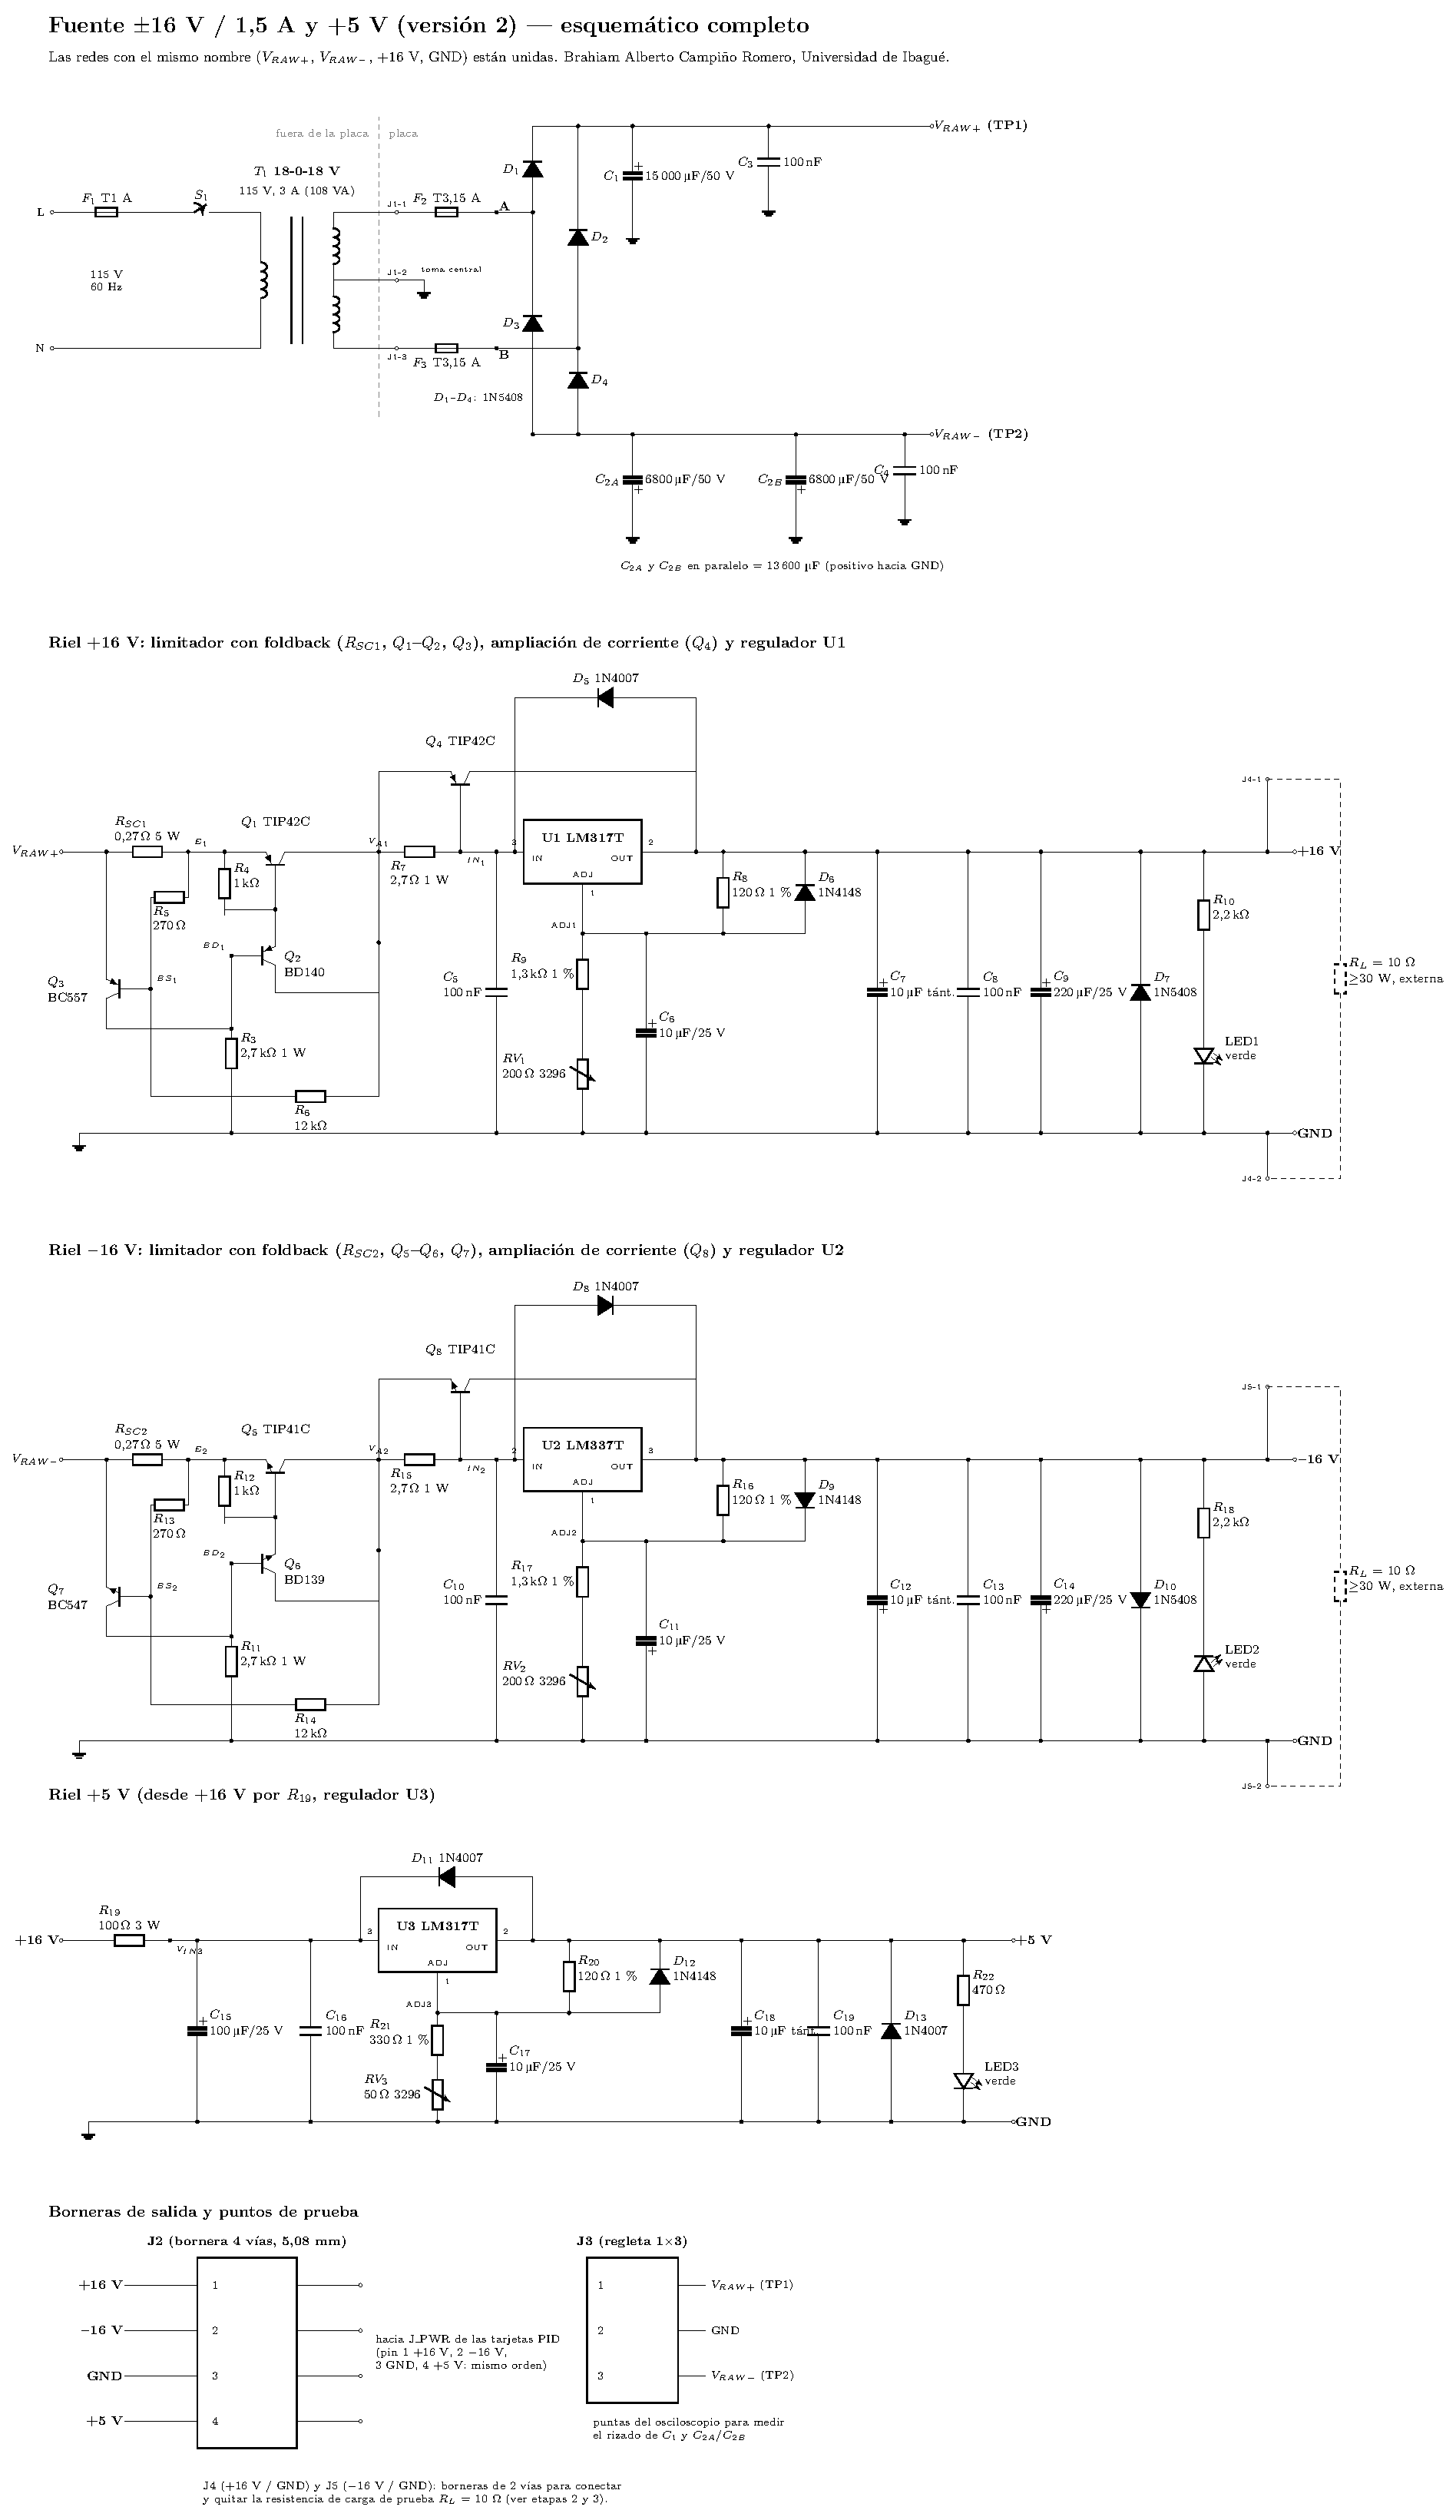
\includegraphics[width=\textwidth,height=0.92\textheight,keepaspectratio]{esq_completo.pdf}
\caption{Esquemático completo de la fuente $\pm$16~V / 1,5~A y +5~V (versión 2).}
\label{fig:completo}
\end{figure*}

\end{document}
